%\documentclass[handout,xcolor=dvipsnames]{beamer}
\documentclass[xcolor=dvipsnames]{beamer}

\usepackage{pgfpages}
%\mode<handout>{\pgfpagesuselayout{4 on 1}[letterpaper,border shrink=5mm,landscape]}
\mode<presentation>{
  \setbeamertemplate{navigation symbols}{}
  %\setbeamertemplate{caption}{\raggedright\insertcaption\par}
  %\setbeamertemplate{caption}[numbered]
}

\usepackage[export]{adjustbox}
\usepackage{graphicx}
\usepackage{algorithm,algorithmic}
\usepackage{multirow}
%\usepackage{cancel}
\usepackage{booktabs} % for midrule
\usepackage{subfig}
\usepackage{tikz}
\usetikzlibrary{shadows,arrows,decorations.pathmorphing,backgrounds,positioning,fit,petri,fadings,shapes,calc,shapes.multipart}

\usepackage{scalefnt}
\usepackage{appendixnumberbeamer}

\usepackage{bbm}
\usepackage{natbib}

\usetheme{Boadilla}

\newcommand{\exclude}[1]{}
\newcommand{\modulus}[1]{\left| #1 \right|}
\newcommand{\norm}[1]{\left\Vert #1 \right\Vert}
\newcommand{\function}[3]{#1 : #2 \mapsto #3}
\newcommand{\real}{\mathbb{R}}
\newcommand{\set}[2]{\left\{ #1 : #2 \right\}}
\newcommand{\ip}[2]{\left< #1 , #2 \right>}
\newcommand{\T}{\mathcal{T}}
\newcommand{\N}{\mathcal{N}}
\newcommand{\I}{\mathcal{I}}
\newcommand{\C}{\mathcal{C}}
\newcommand{\ds}{\displaystyle}
\newcommand{\rec}{\mathrm{rec}}
\renewcommand{\int}[1]{\mathrm{int}(#1)}
\newcommand{\im}[1]{\mathrm{im}(#1)}
\newcommand{\ri}[1]{\mathrm{rint}(#1)}
\newcommand{\dom}[1]{\mathrm{dom}(#1)}
\newcommand{\dual}[1]{#1^D}

\newcommand{\cA}{\mathcal{A}}
\newcommand{\cD}{\mathcal{D}}
\newcommand{\cN}{\mathcal{N}}
\newcommand{\cL}{\mathcal{L}}
\newcommand{\cP}{\mathcal{P}}
\newcommand{\Mu}{\mathcal{M}}

\newcommand{\VI}{\textsc{VI}}
\newcommand{\PATH}{\textsc{Path}}
\newcommand{\EMP}{\textsc{Emp}}
\newcommand{\SELKIE}{\textsc{Selkie}}
\newcommand{\SOL}{\textsc{SOL}}
\newcommand{\st}{\mathrm{s.t.} \hspace*{1pt}}
\newcommand{\Real}{\mathbb{R}\cup\{\infty\}}
\newcommand{\expect}{\mathbb{E}}
\newcommand{\risk}{\rho}
\newcommand{\A}{\mathcal{A}}
\newcommand{\F}{\mathcal{F}}
\newcommand{\cQ}{\mathcal{Q}}
\newcommand{\argmin}{\mathrm{argmin}}
\newcommand{\argmax}{\mathrm{argmax}}
\newcommand{\cvar}{CVaR}
\newcommand{\cvarlo}{\underline{\cvar}}
\newcommand{\cvarup}{\overline{\cvar}}
\newcommand{\Q}{\mathcal{Q}}
\newcommand{\D}{\mathcal{D}}
\newcommand{\EC}{\mathcal{S}}
\newcommand{\black}[1]{{\color{black} #1}}
\newcommand{\red}[1]{{\color{red} #1}}
\newcommand{\blue}[1]{{\color{blue} #1}}
\newcommand{\green}[1]{{\color{OliveGreen!100} #1}}
\newcommand{\purple}[1]{{\color{purple} #1}}
\newcommand{\orange}[1]{{\color{orange} #1}}

%\newcommand{\R}{\Psi}
%\newcommand{\PTDF}{\mathcal{H}}
%\newcommand{\LOOP}{\mathcal{L}}
\newcommand{\MCP}{\text{MCP}}

% \renewcommand{arraystretch}{1.4}
\newenvironment{mytikzpicture}{\noindent\ignorespaces\begin{tikzpicture}}{\end{tikzpicture}\ignorespacesafterend}
\tikzstyle{sensor}=[draw, fill=blue!20, text width=5em, 
    text centered, minimum height=2.5em,drop shadow]
\tikzstyle{ann} = [above, text width=5em, text centered]
\tikzstyle{wa} = [sensor, text width=5em, fill=red!20, 
    minimum height=3em, rounded corners, drop shadow]
\tikzstyle{sc} = [sensor, text width=13em, fill=red!20, 
    minimum height=10em, rounded corners, drop shadow]
\tikzstyle{notimpl}=[draw, semitransparent, fill=blue!20, text width=5em, 
text centered, minimum height=2.5em]%,drop shadow]
\def\blockdist{2}
\def\edgedist{2.5}
\tikzset{vfill/.style={color=black,text=black,fill=red!10!gray!30!blue!50,line width=4pt}}

\title[Werewolf]
{Werewolf and NetZero: the interactions between operations, planning, investments and policies}
\author[Ferris (Wisconsin)]{Michael C. Ferris\\ (Joint work with Josh
  Arnold, Adam Christensen and Andy
  Philpott)}
\institute[]{\alert{Jacques-Louis Lions Chair, and Stephen Kleene Professor of Computer
    Science}\\\alert{Computer Sciences Department and}\\ \alert{Wisconsin Institute for Discovery, University of Wisconsin,
    Madison}}
\date[Thompson CPL support]{Wisconsin Public Utility Institute, Board
  Meeting, \\ Madison, March 10, 2020\\
Supported by Tommy G. Thompson Center on Public Leadership}

\begin{document}
\setbeamertemplate{caption}{\raggedright\insertcaption\par}
%
\begin{frame}
  \titlepage
\end{frame}

\section{Introduction}

\begin{frame}
  \frametitle{Werewolf}

  Who are we, what are we doing.
  
\end{frame}

\begin{frame}
  \frametitle{This talk is about}

  \begin{itemize}
  \item Operations research: helping government policy ...
    \begin{itemize}
    \item to distinguish between objectives and actions;
    \item to understand effects of uncertainty;
    \item to understand effects of incentives.
    \end{itemize}
  \end{itemize}
\end{frame}

\begin{frame}
\frametitle{Simplified two-stage stochastic optimization model}
\begin{itemize}
\item Capacity decisions are $z$ at cost $K(z)$
\item Operating decisions are: generation $y$ at cost $C(y)$,
loadshedding $r$ at cost $Vr$.
\item Random demand is $d(\omega)$.
\item Minimize capital cost plus expected operating cost:
\end{itemize}
\begin{center}
$%
\begin{array}{rrcl}
\text{P:}\quad \displaystyle \min_{(z, y, r) \in X} & \quad K(z)  & + & \expect_{\omega }[%
C(y(\omega )) + Vr(\omega)] \\[1em]
\text{s.t.} & \quad 
\textcolor{black}{y(\omega)} & \textcolor{black}{\leq} & %
\textcolor{black}{z} \\
& \textcolor{black}{y(\omega) + r(\omega)} & \textcolor{black}{\geq} & %
                                                                       \textcolor{black}{d(\omega)}
%\\ &  \alert{z_{\mathcal{N}}} & \leq & \alert{(1-\theta) z_{\mathcal{N}}(2017)}

\end{array}%
$
\end{center}
\begin{itemize}
\item Model populated using data from Wisconsin
\end{itemize}
\end{frame}

\begin{frame}
  \frametitle{Environmental constraints}
Some capacity $z_k$, $k \in \mathcal{N}$, is ``non renewable''.
Some generation $y_k (\omega)$, $k \in \mathcal{E}$ emits $\beta_k y_k
(\omega)$ tonnes of CO2. For a choice of $\theta \in [0, 1]$
constraint is either:
\begin{enumerate}
\item Reduce \alert{CO2 emissions} compared with 2017:
%  \[  \green{\expect_{\omega} [\sum_{k\in \mathcal{E}} \beta_k y_k(\omega)] \leq
%      (1-\theta) \expect_{\omega} [\sum_{k\in \mathcal{E}} \beta_k
%      y_k(\omega,2017)] }
%  \]
\item Reduce \alert{non-renewable capacity} compared with 2017:
%  \[ \blue{\sum_{k\in \mathcal{N}} z_k\leq (1-\theta)  \sum_{k\in
%        \mathcal{N}} z_k(2017) }
%  \]
\item Reduce \alert{non-renewable generation} compared with 2017:
%  \[ \orange{\expect_{\omega} [\sum_{k\in \mathcal{N}} y_k(\omega)] \leq
%      (1-\theta)  \expect_{\omega} [\sum_{k\in \mathcal{N}}
%      y_k(\omega,2017)] }
%  \]
\end{enumerate}
%Could impose constraints almost surely instead of in expectation or
%with risk measure
\end{frame}

\begin{frame}
  % \frametitle{Compare CO2 emissions from reduction strategies}
  \centering
  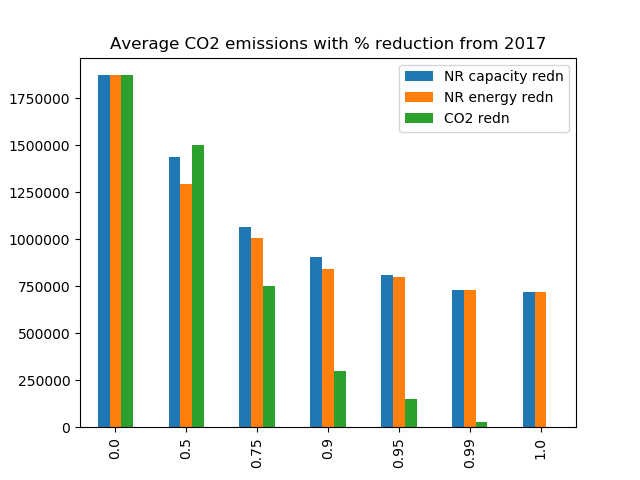
\includegraphics[width=4.0in]{includes/TotalCarbonv20.png} \\
  Since (renewable) geothermal and CCS emit some CO2 100\% renewable yields modest reductions in CO2 emissions.
\end{frame}

\begin{frame}
  % \frametitle{Compare cost of reduction strategies as $\theta$ increases}

  \centering
  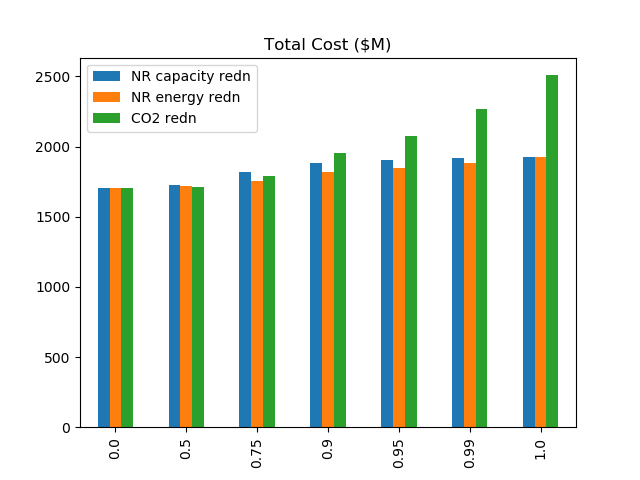
\includegraphics[width=4.0in]{includes/TotalCostMv20.png} \\
  % Increased Electric Vehicle uptake:
  Cost of actually reaching zero CO2 emissions (without geothermal or CCS) increases as we approach the limit.
%\makebox[\linewidth]{\includegraphics[clip,trim=0.1cm 0.2cm 0.1cm
%  1.6cm,page=28,width=5.2in]{OFBPhilpottv2.pdf}}
\end{frame}

\begin{frame}
  \frametitle{Technology choices as $\theta$ increases (NR capacity redn)}

  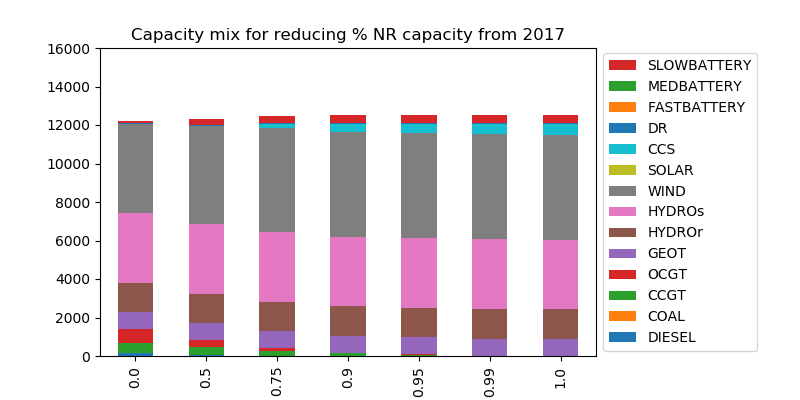
\includegraphics[width=4.8in]{includes/Scaprednv20.png} \\
%\makebox[\linewidth]{\includegraphics[clip,trim=0.1cm 0.2cm 0.1cm
%  1.6cm,page=30,width=5.2in]{OFBPhilpottv2.pdf}}
  \begin{itemize}
  \item Use geothermal, CCS, wind, batteries
  \item Fairly constant capacity
  \end{itemize}
\end{frame}

\begin{frame}
  \frametitle{Technology choices as $\theta$ increases (\% CO2 redn)}

  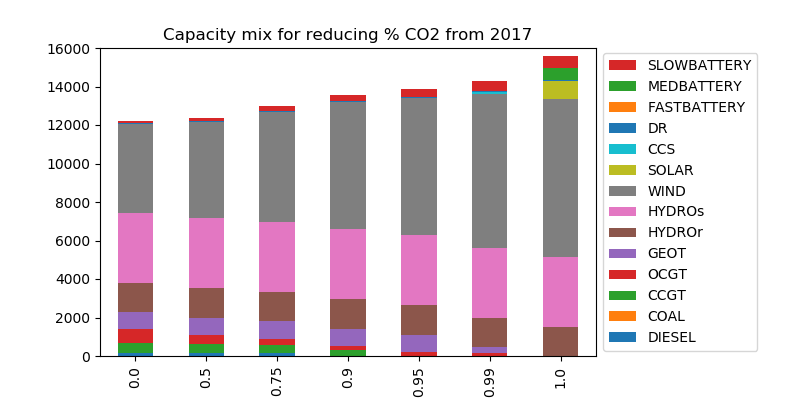
\includegraphics[width=4.8in]{includes/Sco2rednv20.png} \\
%\makebox[\linewidth]{\includegraphics[clip,trim=0.1cm 0.2cm 0.1cm
% 1.6cm,page=30,width=5.2in]{OFBPhilpottv2.pdf}}
  \begin{itemize}
  \item Rich portfolio of renewable technologies used
  \item More capacity needed as more uncertain generation
  \end{itemize}
\end{frame}

\exclude{
\begin{frame}
  \frametitle{Technology choices as carbon price (\$ per MW) increases}

  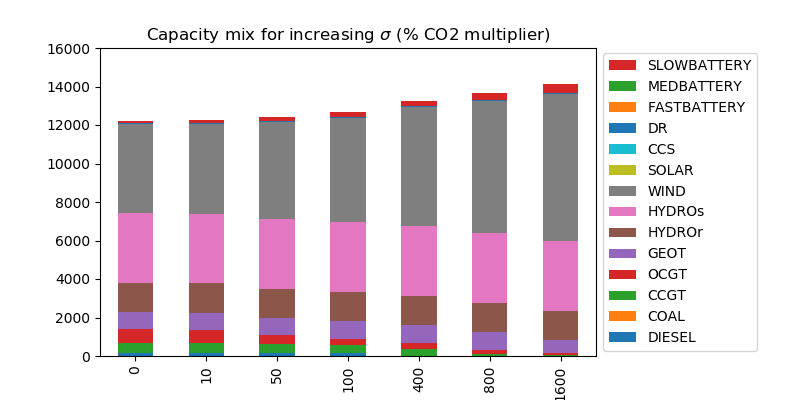
\includegraphics[width=4.8in]{includes/Sco2incrv20.png}
%\makebox[\linewidth]{\includegraphics[clip,trim=0.1cm 0.2cm 0.1cm
%  1.6cm,page=30,width=5.2in]{OFBPhilpottv2.pdf}}
\end{frame}

\begin{frame}
  \frametitle{CO2 reduction (constraint or carbon tax)}

    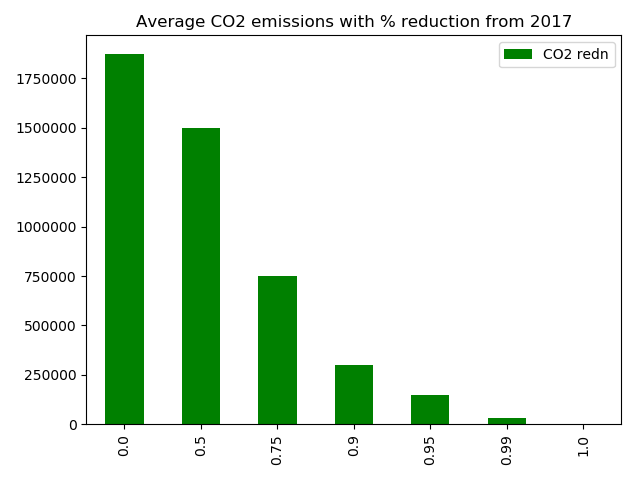
\includegraphics[width=0.5\textwidth]{includes/TotalCarbonSinglev20.png}
    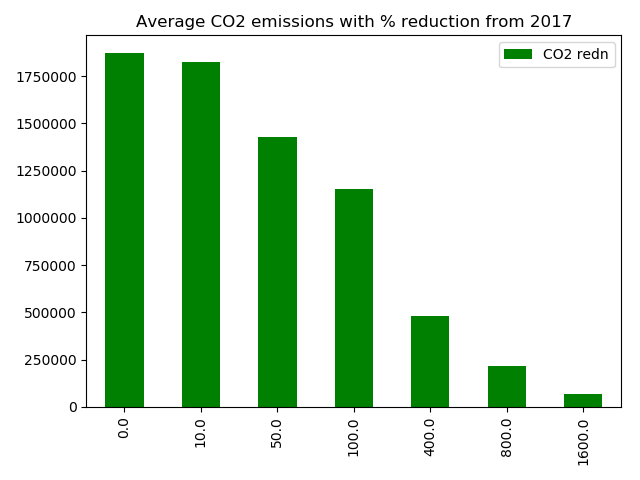
\includegraphics[width=0.5\textwidth]{includes/TotalCarbonincrv20.png}

\end{frame}
}

\begin{frame}
  \frametitle{Carbon emissions (almost sure)}

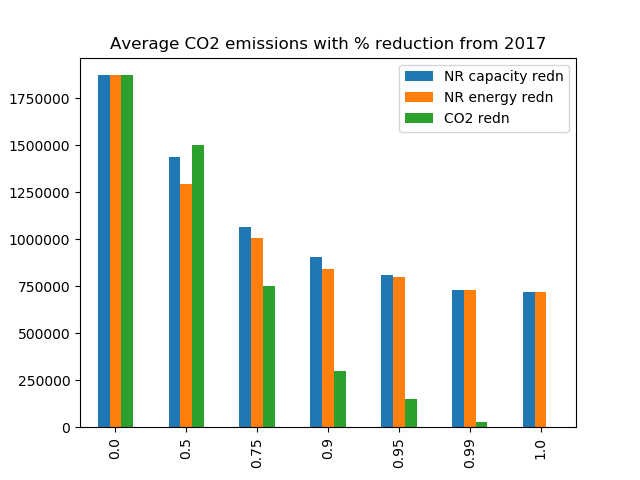
\includegraphics[width=0.5\textwidth]{includes/TotalCarbonv20.png}
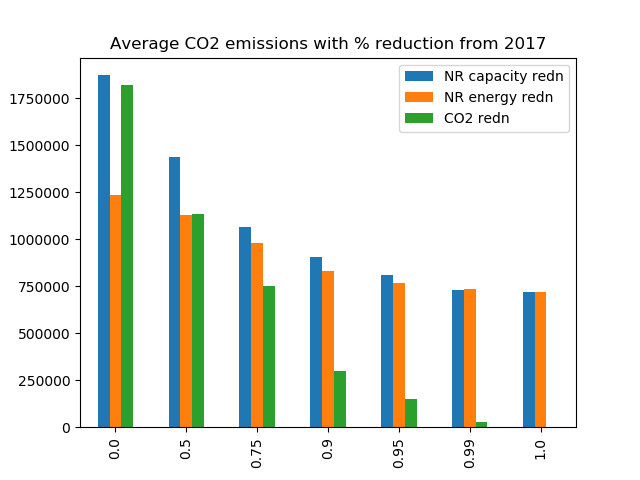
\includegraphics[width=0.5\textwidth]{includes/TotalCarbonASv20.png}

\begin{itemize}
\item Average reduction, vs reduction {\em in every scenario}
\item Significant differences only at relatively low levels of CO$_{2}$
reduction
\item Single year, 2005, in which the emissions are significantly higher
than all the others in the average case, but is compensated for by
reduced emissions in other  years.
\end{itemize}
\end{frame}

\exclude{
\begin{frame}
  \frametitle{Technologies (chance constraints):
    cf. increased uptake}

\centering
Force zero emissions in at least 50\% of years (normal hydrology)\\
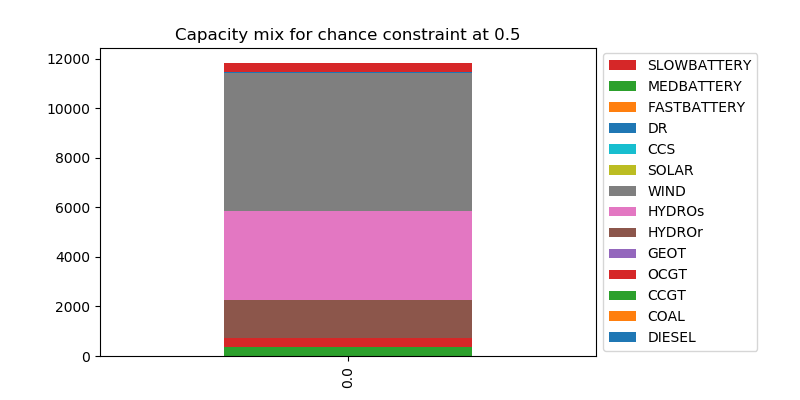
\includegraphics[clip,trim=1.25cm 0.95cm 0.0cm 0.0cm,height=2.8cm]{includes/SccConstraint.png}
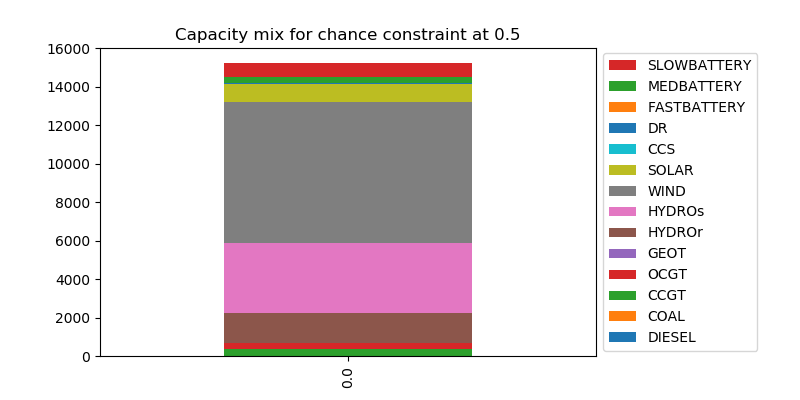
\includegraphics[clip,trim=1.25cm 0.95cm 5.1cm 0.0cm,height=2.8cm]{includes/SccConstraintv20.png}\\
  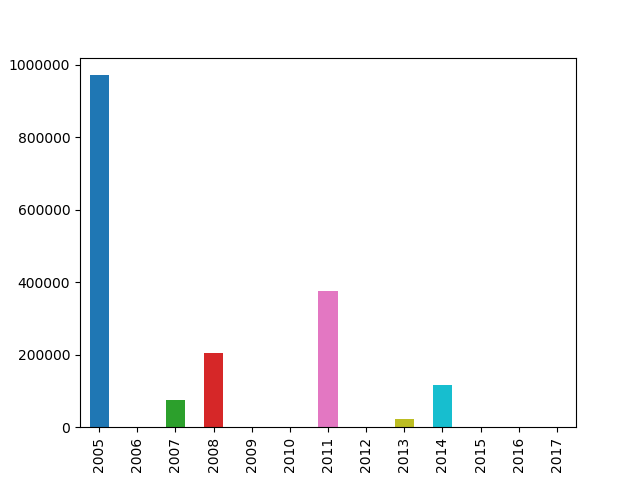
\includegraphics[width=0.4\textwidth]{includes/CCvalues.png}\qquad
  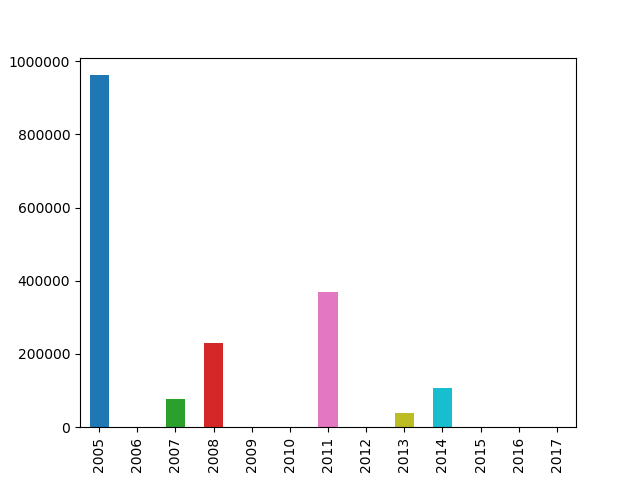
\includegraphics[width=0.4\textwidth]{includes/CCvaluesv20.png}\\

  Nonzero CO$_{2}$ emissions in 6 out of the 13 scenarios\\
  Average level of CO$_{2}$ emissions (0.138 Mt) or approx 95.4\% redn

\end{frame}
}

\begin{frame}
  \frametitle{Conclusions}
  \begin{itemize}
  \item Models can inform policy
  \item Models can show effects and costs of constraints
  \item Investment is coupled to reliability
  \item \color{black} Very large scale models (many agents with many instruments
    acting strategically) with risk are hard
  \item \alert{New algorithms enable solution of more detailed,
      authentic problems and address underlying policy questions}
  \item Evaluation via simulation computations and out-of-sample testing
  \end{itemize}
\end{frame}

\end{document}
